\section{Diagnostics with Toys}
\label{sec:toys}

Frequentest statistical methods usually involve the generation of many pseudo-datasets (toys) in order to 
evaluate the distribution of some parameter or test statistic. These distributions are used to set
confidence intervals or determine the significance of some observed excess from experimental data.
The Higgs searches at CMS use the profile likelihood test statistic (Equation~\ref{eqn:llr}) in which
the nuisance parameters (${\theta}$) are profiled (fit) from the data. (Details of the modelling 
of systematic uncertainties through nuisance parameters can be found in~\cite{CMS-11-032}).

For calculating the significance of an excess observed in data, it is necessary to evaluate the distribution 
of the test statistic $q_{0}$. This is the distribution of the test statistic in the absence of signal or under the
background only hypothesis. At CMS, the test statistic $q_{0}$ is modified so that $q_{0}=0$ when $\hat{\mu}<0$ so as
to report only excesses in the data over the background. The procedure for determining this distribution proceeds as follows;

\begin{itemize}
\item{Fit the observed data fixing $\mu=0$. The values of the nuisance parameters 
at which the likelihood attains its maximum are denoted $\theta_{obs}$ and will represent the expectation value of the nuisance
parameters in the likelihood.}
\item{Generate a toy dataset under the background only hypothesis. For the purposes of
generating data, the nuisance parameters are fixed to $\theta=\theta_{obs}$.}
\item{Fit the toy dataset twice, once fixing $\mu=0$, $\call(data|0,\hat{\theta}_{0})$ and once more letting 
$\mu$ float freely, $\call(data|\hat{\mu},\hat{\theta})$. For the purposes of 
evaluating the likelihood, the values $\theta_{obs}$ are randomized in order to model the systematic uncertainty.}
\end{itemize}

\subsection{Realistic Counting Experiment}
An realistic example of a search for an hypothesised particle, $H$, decaying to two $\tau$ leptons was produced in the form 
of a simple counting experiment. The search is performed as a combination of three channels arising from the possible subsequent 
decays of the two $\tau$ leptons; $\tau_{h}-e$, $\tau_{h}-\mu$ and $e-\mu$. In each channel the expected background is known with
some degree of certainty either from simulation or some control region in data. The observed data in each channel is represented 
by a count of events. 
Several sources of systematic uncertainty are included which effect the expected signal and background in one or more of the channels. 
Systematics are incorporated into the likelihood in the form of nuisance parameters.

The analysis is summarized in Table~\ref{tab:realanalysis}. The number of expected events from each background process and the number of
expected signal events is given for each channel. The number of observed events is also given per channel. Systematics which effect
more than one process or channel are treated as 100\% correlated across those channels.

\begin{table}
\centering
\begin{tabular}{|l|c|c|c|c|c|c|c|c|c|}
\hline
\textbf{channel} & \multicolumn{3}{c|}{$\tau_{h}-e$} & \multicolumn{3}{|c|}{$\tau_{h}-\mu$} &\multicolumn{3}{c|}{$e-\mu$}   	\\ \hline
observed & \multicolumn{3}{c}{517} &\multicolumn{3}{|c|}{540} & \multicolumn{3}{c|}{101} 				\\ \hline
expected & Sig & $Z\tau\tau$ & QCD & Sig & $Z\tau\tau$ & QCD &Sig & $Z\tau\tau$ & other 				\\ \hline
	 & 0.34 & 190 & 327 &  0.57 & 329 & 259 & 0.15 & 88 & 14							\\ \hline
\hline
\textbf{systematics} & \multicolumn{9}{c|}{} \\ \hline
lumi	 & 11\% & - & - & 11\% & - & - & 11\% & - & 11\% 	\\ \hline 
tauid	 & 23\% & 23\% & - & 23\% & 23\% & - & - & - & -  	\\ \hline 
ZtoLL    & - & 4\% & - & - & 4\% & - & - & 4\% & - 		\\ \hline
effic    & 4\% & 4\%&  - & 4\% & 4\% & - & 4\% & 4\% & 4\%	\\ \hline  
QCDel	 & - & - & 20\% & - & - & - & - & - & - 		\\ \hline
QCDmu    & - & - & - & - & - & 10\% & - & - & -			\\ \hline
other    & - & - & - & - & - & - & - & - & 10\%			\\ \hline
\end{tabular}
\caption{A realistic counting experiment across several channels. The number of observed events and that expected from signal and background
processes are given per channel. Several sources of systematic are included which effect the expected rate of each signal or background process. 
Where a dash is entered, the systematic uncertainty has no effect on that process or channel. \label{tab:realanalysis}}
\end{table}

The analysis was coded into a \texttt{RooFit} workspace using the \texttt{CMSSW} package \\
\texttt{HiggsAnalysis/CombinedLimit}\\
from the datacard provided under \\ \texttt{data/tutorials/realistic-counting-experiment.txt}.

The package is used to provide a likelihood which encodes all aspects of the analysis and tools for generating toy datasets and
fitting to them. Details about the version of the code used can be found in~\ref{sec:versions}. Around 90,000 toy datasets were generated and fitted
using the tool \texttt{MaxLikelihoodFit}. The toys were generated under the background only hypothesis as is appropriate to determine the 
distribution of $q_{0}$ (setting $\mu$ of Equation~\ref{eqn:llr} to zero).
Each toy dataset was fit twice, once fixing the signal strength, $\mu$, to zero and a second allowing $\mu$ to float freely.
The results of the fits are saved to \texttt{TTree} objects which can then be used to diagnose the fits and highlight potentially problematic
channels or nuisance parameters. These can be summarized using the tool \texttt{plotParametersFromToys}. 

Figure~\ref{fig:real_lumi_s} shows the summary of the nuisance parameter \texttt{lumi}, which models the systematic associated to uncertainty 
of the total luminosity of the dataset, from the signal plus background fits to the toys.
The upper left panel shows two pull distributions of the values from the fit defined as the difference between the value of the fitted parameter
and the value from the best fit to data, $\theta_{obs}$, divided by the error on the parameter (usually close to 1 for most systematics). 
The blue histogram includes all toys while the red shows the results
only for which the best fit signal strength is positive. Since the test-statistic $q_{0}$ is designed to report only excesses in the data,
it is important to check that nuisance parameters correlated to the signal strength are well-behaved.

The pull distributions are fitted with a Gaussian and the width and mean are reported in the upper right panel. Since the constrain terms in the 
likelihood for nuisances are generated around the best fit to data, the pulls are expected to be centered around 0. In general, the nuisance parameters
are constrained from external measurements ans so it is expected that the width of the pull distribution is 1. Nuisance parameters which are further
constrained by the observed data will typically have a pull distribution with width $<$1. The parameter \texttt{lumi} does not show signs of being constrained
by the data. This is reflected in the lower left panel which shows a scatter plot of the expectation value in each toy versus the fitted value of that 
nuisance. This behaviour is expected since this nuisance parameter mostly effects the signal process and is correlated across all channels so that only the overall
normalization is altered. Since these fits allow $\mu$ to float freely, any parameter which alters only the overall normalization of the signal should achieve its 
expectation value at the maximum of the likelihood. 

The lower right panel shows the shape of the negative log-likelihood projected along the axis of the nuisance parameter near the maximum 
of the likelihood. At each point, all other parameters are fixed to those of the best fit to the data (in this case, from the fit allowing $\mu$ to float).
The likelihood is expected to be parabolic around its minima with no secondary (local) minima present. This panel can be used to check if the true global 
minima was found in the fit to data. A similar summary plot is shown for the fits in which $\mu$ is fixed to 0 in Figure~\ref{fig:real_lumi_b}


\begin{figure*}[hbtp]
  \begin{center}
    \subfigure[][]{
    	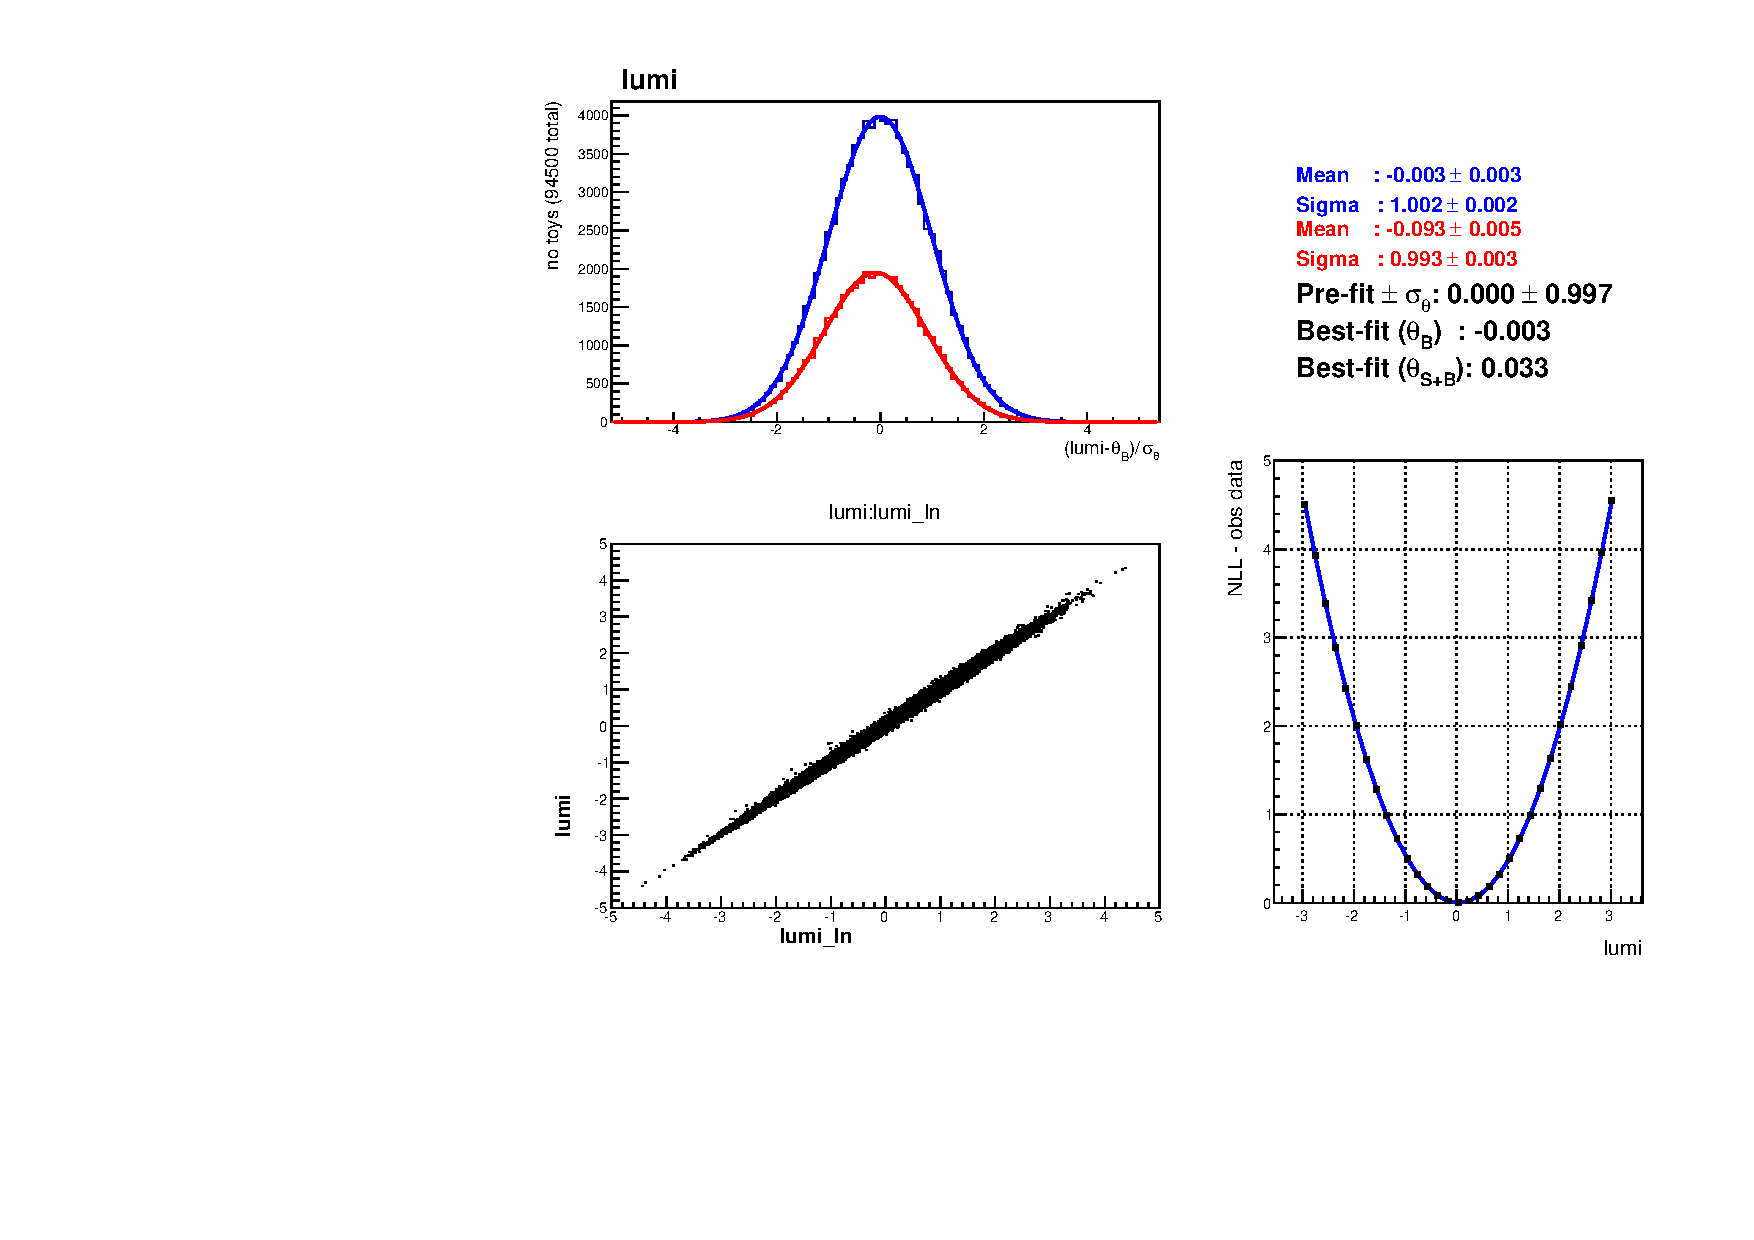
\includegraphics[width=0.85\textwidth]{figures/tree_fit_sb_lumi.pdf}
	\label{fig:real_lumi_s}
    }\\
    \subfigure[][]{
    	\includegraphics[width=0.85\textwidth]{figures/tree_fit_b_lumi.pdf}
	\label{fig:real_lumi_b}
    }\\
    \caption{Summary plots for the parameter \texttt{lumi} of the realistic counting experiment. Both signal plus background (a) and 
background only (b) fits are shown. The toys are generated under the background only hypothesis by setting $\mu=0$}
  \end{center}
\end{figure*}


Figure~\ref{fig:real_tauid_s} shows the summary plots for the nuisance parameter \texttt{tauid} which models the systematic related to uncertainty in the
efficiency for identifying an hadronically decaying $\tau$. This nuisance parameter is correlated across the signal and one of the background processes
in two channels. This is reflected in the fits as the fitted parameter is not 100\% correlated with the value drawn for the expectation in the likelihood
(as seen in the spread in the scatter plot in the lower left panel).
This parameter is strongly constrained from the observed data since small changes in this parameter contribute significantly to the likelihood.
This is also seen in the pull distributions as they exhibit a width $<$1. Behaviour such as this can indicate that an uncertainty is over-estimated or
only weakly constrained from the external measurements. A summary of the pulls for all of the nuisance parameters is given in 
Figures~\ref{fig:real_pulls_s} and~\ref{fig:real_pulls_b}.
The error bars denote the width of the pull distribution for each parameter. Nuisances which are strongly constrained by the data will have a width $<$1 sigma.

\begin{figure*}[hbtp]
  \begin{center}
    \subfigure[][]{
    	\includegraphics[width=0.85\textwidth]{figures/tree_fit_sb_tauid.pdf}
	\label{fig:real_tauid_s}
    }\\
    \subfigure[][]{
    	\includegraphics[width=0.85\textwidth]{figures/tree_fit_b_tauid.pdf}
	\label{fig:real_tauid_b}
    }\\
    \caption{Summary plots for the parameter \texttt{tauid} of the realistic counting experiment. Both signal plus background (a) and 
background only (b) fits are shown. The toys are generated under the background only hypothesis by setting $\mu=0$}
  \end{center}
\end{figure*}

\begin{figure*}[hbtp]
  \begin{center}
    \subfigure[][]{
    	\includegraphics[width=0.85\textwidth]{figures/real_pulls_s.png}
	\label{fig:real_pulls_s}
    }\\
    \subfigure[][]{
    	\includegraphics[width=0.85\textwidth]{figures/real_pulls_b.png}
	\label{fig:real_pulls_b}
    }\\
    \caption{Pull summary plots for the nuisance parameters of the realistic counting experiment. The central point marks the mean of a Gaussian fitted to 
the pull distribution and the error bar represents the width of the Gaussian. Both signal plus background (a) and background only (b) fits are shown.}
  \end{center}
\end{figure*}

\subsection{CMS Higgs Search 2011+2012 Combination}

The diagnostic tools for use with toys were run over the combined search described in Section~\ref{sec:data}.
Around 10,000 toys were generated for $m_{H}=125~GeV$ under the background only hypothesis, $\mu=0$, as is appropriate for 
building the distribution of the test-statistic $q_{0}$ used for quantifying excesses in observed experimental data. Figure~\ref{fig:combination_hww_wwbounding_b} is an example of the diagnostic plots from a typical nuisance parameter 
of the $H\rightarrow WW$ analysis,\\ 
\texttt{CMS\_hww\_MVAWWBounding}. The upper left panel shows the pull distribution for the fitted parameter. The width of
the pull is $<1$ indicating that this parameter is further constrained by the data. This can
also be seen in the lower left panel as the fitted parameter shows only some correlation with the expectation value. 

\begin{figure*}[hbtp]
  \begin{center}
    	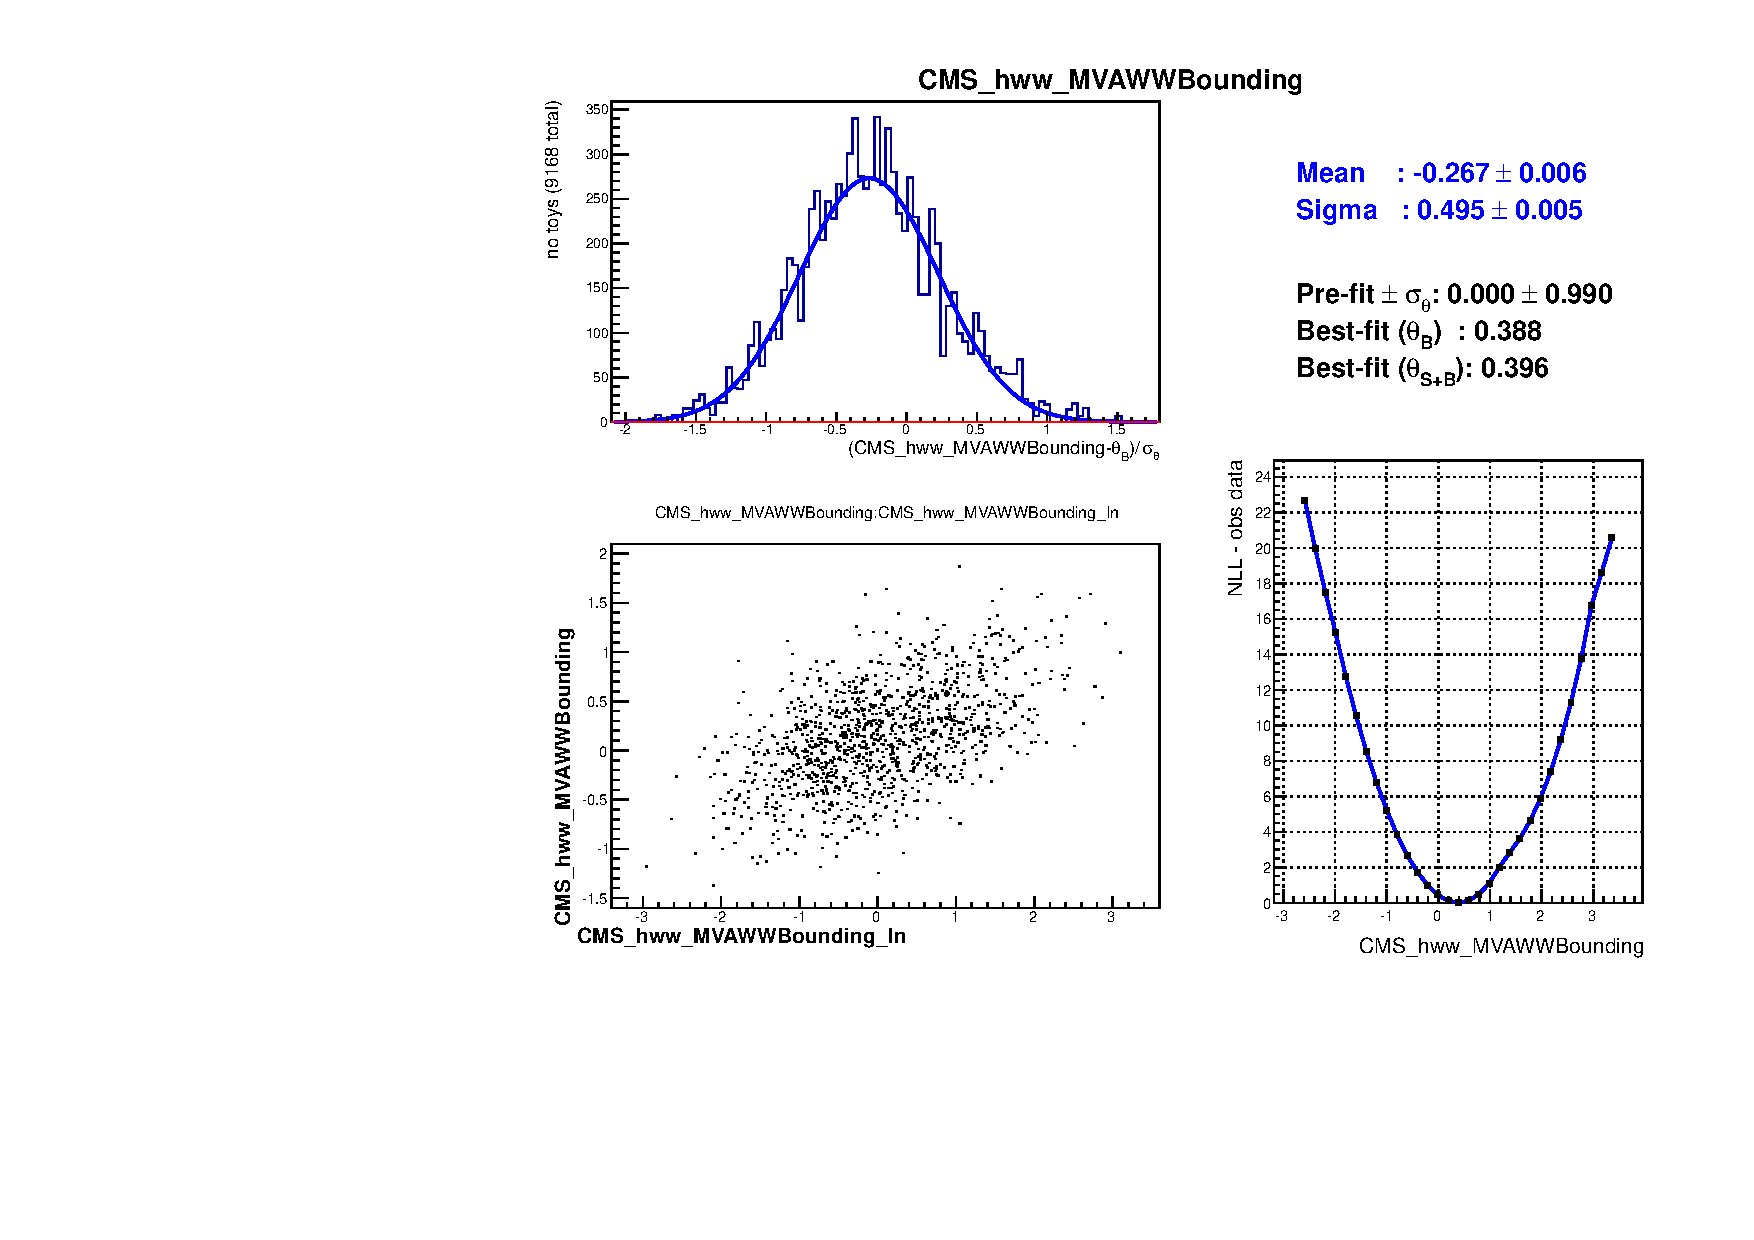
\includegraphics[width=0.85\textwidth]{figures/tree_fit_b_CMS_hww_MVAWWBounding.pdf}
    \caption{Summary plots for the parameter \texttt{CMS\_hww\_MVAWWBounding}. 
The entries in the histograms are for fits to background only toys letting $\mu$ float freely\label{fig:combination_hww_wwbounding_b}.}
  \end{center}
\end{figure*}

This nuisance parameter only effects the $qq\rightarrow WW$ signal in the 2011 
$H\rightarrow WW \rightarrow l\nu l\nu$ MVA shape analysis in the $0-jet$ and $1-jet$ categories. The effect of the uncertainty 
is modelled using template morphing. This is achieved by providing histograms which represent the nominal distribution and 
the distribution resulting from $\pm1\sigma$ deviations of the nuisance parameter, for each category as shown in 
Figure~\ref{fig:hww_templates_qqww_wwbounding}. 

\begin{figure*}[hbtp]
  \begin{center}
    	\includegraphics[width=0.45\textwidth]{figures/wwof0j_wwbounding}
    	\includegraphics[width=0.45\textwidth]{figures/wwof1j_wwbounding}\\
    	\includegraphics[width=0.45\textwidth]{figures/wwsf0j_wwbounding}
    	\includegraphics[width=0.45\textwidth]{figures/wwsf1j_wwbounding}\\
    \caption{Templates representing the variation in MVA output shape of the $qq\rightarrow WW$ signal from the $H\rightarrow WW$ 2011 analysis resulting
from systematic variation of the parameter \texttt{CMS\_hww\_MVAWWBounding}. The upper left/right plots show the templates for the opposite flavour lepton
categories while the lower left/right plots show the same flavour lepton categories\label{fig:hww_templates_qqww_wwbounding}.}
  \end{center}
\end{figure*}

A summary of the pulls from all of the nuisance parameters from this combination and some example diagnostic plots can be found in Section~\ref{app:combinationpulls}.

%\begin{table}[hbt!]
%\centering
%\begin{tabular}{|l|r|r|r|} \hline 
%                                         &     $b$-only fit &       $s+b$ fit &        \\
%name                                     &  $\Delta x/\sigma_{\text{in}}$, $\sigma_{\text{out}}/\sigma_{\text{in}}$ & $\Delta x/\sigma_{\text{in}}$, $\sigma_{\text{out}}/\sigma_{\text{in}}$ & $\rho(\theta, \mu)$ \\  \hline
%QCDel                                    &  {{\color{red}\textbf{ +0.30, 0.41}}} & {{\color{red}\textbf{ +0.31, 0.41}}} &  -0.01 \\
%QCDmu                                    &      -0.27, 0.91 &     -0.23, 0.91 &  -0.01 \\
%ZtoLL                                    &      -0.10, 0.94 &     -0.01, 0.94 &  -0.03 \\
%effic                                    &      -0.11, 0.93 &     +0.00, 0.93 &  -0.03 \\
%lumi                                     &      -0.00, 0.99 &     +0.03, 0.99 &  -0.01 \\
%other                                    &      -0.00, 0.99 &     +0.03, 0.99 &  -0.01 \\
%tauid                                    &  {{\color{red}\textbf{ -0.51, 0.50}}} & \textbf{ -0.41, 0.50} &  -0.06 \\
% \hline
%\end{tabular}
%\label{tab:realnuisdiff}
%\end{table}
